\documentclass[hyperref,UTF-8]{ctexart}
\usepackage{ctex}
\usepackage[dvipsnames,svgnames]{xcolor}
\usepackage{newtxtext}
\usepackage{lipsum}
\usepackage[strict]{changepage}
\usepackage{framed}
\usepackage{graphicx}
\usepackage{float}
\usepackage{geometry}
\usepackage{amsmath}
\usepackage{tcolorbox}
\usepackage{amssymb}
\usepackage{mathrsfs}
\usepackage{cite}
\usepackage{bm}
\usepackage[colorlinks,linkcolor = Black]{hyperref}
\newcommand{\R}{\mathbb{R}}
\newcommand{\F}{\mathbb{F}}
\newcommand{\N}{\mathbb{N}}
\newcommand{\Q}{\mathbb{Q}}
\newcommand{\Z}{\mathbb{Z}}
\newcommand{\E}{\text{E}}
\newcommand{\Cov}{\text{Cov}}
\newcommand{\0}{\boldsymbol{0}}
\newcommand{\setparDis}{\setlength{\parskip} {0.3cm} }
\tcbuselibrary{most}
\definecolor{examplecolor}{rgb}{0.77,0.72,0.65} % 莫兰迪棕色
% ------------------******-------------------
\newtcolorbox{example}[2][]
{enhanced,breakable,
left=12pt,right=12pt,% 左右边距
% fonttitle=\bfseries, % 可以设置标题是否粗体
coltitle=white, % 标题字体颜色
colbacktitle=examplecolor, % 标题背景颜色
attach boxed title to top left={yshifttext=-1mm},
boxed title style={skin=enhancedfirst jigsaw,arc=1mm,bottom=0mm,boxrule=0mm},
boxrule=1pt, % 边框线宽
%
colback=OldLace, % 文本框背景颜色
colframe=examplecolor, % 框线颜色
%
sharp corners=northwest,
% drop fuzzy shadow, % 可以选择是否设置阴影效果
title=\vspace{3mm}#2,
arc=1mm,
#1}%

\newtcolorbox{justification}[2][]
{enhanced,breakable,
left=12pt,right=12pt,% 左右边距
% fonttitle=\bfseries, % 可以设置标题是否粗体
coltitle=white, % 标题字体颜色
colbacktitle=BurntOrange, % 标题背景颜色
attach boxed title to top left={yshifttext=-1mm},
boxed title style={skin=enhancedfirst jigsaw,arc=1mm,bottom=0mm,boxrule=0mm},
boxrule=1pt, % 边框线宽
%
colback=white, % 文本框背景颜色
colframe=BurntOrange, % 框线颜色
%
sharp corners=northwest,
% drop fuzzy shadow, % 可以选择是否设置阴影效果
title=\vspace{3mm}#2,
arc=1mm,
#1}%

\newtcolorbox{understanding}[2][]
{enhanced,breakable,
left=12pt,right=12pt,% 左右边距
% fonttitle=\bfseries, % 可以设置标题是否粗体
coltitle=white, % 标题字体颜色
colbacktitle=RoyalBlue, % 标题背景颜色
attach boxed title to top left={yshifttext=-1mm},
boxed title style={skin=enhancedfirst jigsaw,arc=1mm,bottom=0mm,boxrule=0mm},
boxrule=1pt, % 边框线宽
%
colback=white, % 文本框背景颜色
colframe=RoyalBlue, % 框线颜色
%
sharp corners=northwest,
% drop fuzzy shadow, % 可以选择是否设置阴影效果
title=\vspace{3mm}#2,
arc=1mm,
#1}%

\newtcolorbox{definition}[2][]
{enhanced,breakable,
left=12pt,right=12pt,% 左右边距
% fonttitle=\bfseries, % 可以设置标题是否粗体
coltitle=white, % 标题字体颜色
colbacktitle=Green, % 标题背景颜色
attach boxed title to top left={yshifttext=-1mm},
boxed title style={skin=enhancedfirst jigsaw,arc=1mm,bottom=0mm,boxrule=0mm},
boxrule=1pt, % 边框线宽
%
colback=white, % 文本框背景颜色
colframe=Green, % 框线颜色
%
sharp corners=northwest,
% drop fuzzy shadow, % 可以选择是否设置阴影效果
title=\vspace{3mm}#2,
arc=1mm,
#1}%
\definecolor{blueshade}{rgb}{0.95,0.95,1} % 蓝色文本框,竖线颜色设为 RoyalBlue
\definecolor{greenshade}{rgb}{0.90,0.99,0.91} % 绿色文本框,竖线颜色设为 Green
\definecolor{redshade}{rgb}{1.00,0.90,0.90}% 红色文本框,竖线颜色设为 LightCoral
\definecolor{brownshade}{rgb}{0.99,0.97,0.93} % 棕色文本框,竖线颜色设为 BurlyWood


\newenvironment{brownformal}{%
\def\FrameCommand{%
\hspace{1pt}%
{\color{BurlyWood}\vrule width 2pt}%
{\color{brownshade}\vrule width 4pt}%
\colorbox{brownshade}%
}%
\MakeFramed{\advance\hsize-\width\FrameRestore}%
\noindent\hspace{-4.55pt}% disable indenting first paragraph
\begin{adjustwidth}{}{7pt}%
\vspace{2pt}\vspace{2pt}%
}
{%
\vspace{2pt}\end{adjustwidth}\endMakeFramed%
}

\newenvironment{blueformal}{%
\def\FrameCommand{%
\hspace{1pt}%
{\color{RoyalBlue}\vrule width 2pt}%
{\color{blueshade}\vrule width 4pt}%
\colorbox{blueshade}%
}%
\MakeFramed{\advance\hsize-\width\FrameRestore}%
\noindent\hspace{-4.55pt}% disable indenting first paragraph
\begin{adjustwidth}{}{7pt}%
\vspace{2pt}\vspace{2pt}%
}
{%
\vspace{2pt}\end{adjustwidth}\endMakeFramed%
}

\hypersetup{
colorlinks = true,
linkcolor = Black,
filecolor = Black,
bookmarks = true,
urlcolor = RoyalBlue,
citecolor = cyan,
bookmarksopen = false,
pdfpagemode = FullScreen,
pdfstartview = Fit
}
\CTEXsetup[format={\bfseries}]{section}
\CTEXsetup[format={\bfseries}]{subsection}


\geometry{a4paper,left = 2cm, right = 2cm, top = 2cm, bottom = 2cm}

\linespread{1.7}
\begin{document}
\setparDis

\begin{titlepage}
    \centering

    %------------------------------------------------------------
    %    Top rules
    %------------------------------------------------------------

    \rule{\textwidth}{1pt}   % The top horizontal rule
    \vspace{0.2\textheight}  % Whitespace between top horizontal rule and title

    %------------------------------------------------------------
    %    Title
    %------------------------------------------------------------

    {\Huge Notes for Statistical Mechanics}

    \vspace{0.025\textheight}   % Whitespace between the title and short horizontal rule

    \rule{0.83\textwidth}{0.4pt}  % The short horizontal rule under title

    \vspace{0.1\textheight}  % Whitespace between the short horizontal rule and author

    %------------------------------------------------------------
    %    Author
    %------------------------------------------------------------

    {\Large \textsc{\kaishu 禤科材}}

    \vspace{0.015\textheight}

    {\Large \textsc{\kaishu 中国科学技术大学\;化学物理系}}

    \vfill  % Whitespace between author and date

    {\large \kaishu 2023年7月1日}
    \vspace{0.1\textheight}  % Whitespace between date and bottom horizontal rule

    %------------------------------------------------------------
    %    Bottom rules
    %------------------------------------------------------------

    \rule{\textwidth}{1pt}  % The bottom horizontal rule

  \end{titlepage}


\nocite{*}

\tableofcontents

\pagebreak
\fontsize{12pt}{16pt}

\section{前言}

统计力学将热力学问题归结于 \textcolor{RoyalBlue}{\textbf{\kaishu 概率与统计推断}},以等概率假设与遍历性假设为基础,建立起一整套关于微观-宏观相互联系的桥梁。通过一定的统计推断,我们可以从众多自由度中提取出一些重要信息,而忽视一些细节,或者无关紧要的部分\cite{suyu}。

虽然我们打算忽略一些细节,但是还是得来看看这些细节都是怎么一回事。经典力学以相空间和哈密顿函数为基础,以\textcolor{RoyalBlue}{\textbf{\kaishu 正则变量}} 的时间演化给出力学系统的时间演化。这些正则变量服从哈密顿方程:
\begin{align}
    \dot{q_i} &= \frac{\partial H}{\partial p_i} \\
    \dot{p_i} &= -\frac{\partial H}{\partial q_i}
\end{align}
不过,要想求解如此庞大的耦合微分方程系统是很困难的一件事——例如采样,而且是对 $10^{23}$ 量级的粒子数!既然庞加莱早已证明,连最简单的三体问题都没有解析解,且对初值敏感, \textcolor{RoyalBlue}{\textbf{ \kaishu 我们又有什么信心认为对于 $10^{23}$ 量级的结果是可靠的呢?}}

好消息是,统计力学的遍历性假设将会让这些烦人的细节从我们的面前消失。考虑一个宏观小而微观大的子系统,它与周围的环境进行着复杂紊乱的相互作用,所以我们有理由认为:在足够长的时间间隔内子系统在自身所有可能的状态中经历足够多的次数\cite{lan}。同时,这一假设也让我们相信:某个子系统的统计分布与同一系统的其他任意小部分的初始状态无关,因为从任何初始状态出发,这个系统总是将所有可能的状态都走了足够多遍,以至于这种初始状态的影响在足够长的时间内,被系统其余的、更为广大的部分的影响所完全消除。换句话说, \textcolor{RoyalBlue}{\textbf{\kaishu 每一个状态都可以取为初始状态}} 。

所以我们看到,统计力学对一个物理系统的预言具有概率的特征。但必须指出的一点是,这样的概率绝非系统所固有,而是因为得到这些结论所依据的条件远比完整的力学描述所需要的少得多——例如我们可以仅用三个宏观可测的状态参量就能完全确定一个宏观系统,还能确定系统其他的状态参量的值,而这三个自由度实际上将天文数字的微观自由度都统摄其下。

另一个问题是 \textcolor{RoyalBlue}{\textbf{\kaishu 微观可逆性与宏观不可逆性的矛盾 }}——如果用 $-t$ 替代求解结果中的 $t$ (做一个时间反演,或者说把录像带倒着放)仍然是演化方程的一个可能的解,但我们从来没有观察到滴进池塘的墨水又重新聚集成刚滴进去时的形状。这样一来, \textcolor{RoyalBlue}{\textbf{\kaishu 时间的流逝似乎就有了确定的方向。}} 这样的“热力学时间”和我们其他地方作为正则变换参量(Hamilton-Jacobi 理论)或者酉变换参量(量子力学传播子)所引入的时间有什么差别?

总之,统计力学是作者本科以来最喜欢的一门理论课,它是一个关于“大”的理论。固然对“小”的研究也同样迷人(量子力学、第一性原理计算、单分子反应机理的探究等等),对这些细节的研究加深了我们对自然界的微观认识,使得我们对自然界究竟是怎样运转的有了更多的了解,甚至能在原子、电子、夸克尺度上让基本力服从我们的意志,但它能指引我们走多远呢?世界的本源有小有大,而我选择相信 \textcolor{RoyalBlue}{\textbf{\kaishu More Is Different}}。具有巨大自由度数目的系统虽然系统与单一粒子遵循同样的力学规律,但是自由度的巨大却导致性质上的全新规律性。而这样的规律,是在微观层面意识不到的。

不识庐山真面目,只缘身在此山中。进入大数据时代,甚至现在的 new bing 和 ChatGPT 所引领的大语言模型时代,科学界的主要矛盾也在变化。这是统计模型大放光彩的时代,也是科技革命的浪潮之巅。

统计力学将会爆发出的能量,我想是不言而喻的。

\pagebreak 


\section{系综理论的基本原理}

经典力学通过相空间中的点 $(q,p)$ 来描述一个系统的某个状态。它们的演化满足正则方程
\begin{align*}
    \dot{q_i} &= \frac{\partial H}{\partial p_i} \\
    \dot{p_i} &= -\frac{\partial H}{\partial q_i}
\end{align*}
现在,我们想要考虑的不是一个状态,而是一大群状态——  \textcolor{RoyalBlue}{\textbf{\kaishu 在单一瞬间同时考虑大量系统,他们全部是给定系统的某种“思维复本”——其特性由与原系统一样的宏观态来表征,但极其自然地处在所有各种可能的微观态中}} \cite{Pathria}。

所以,所谓系综是这样一个集合,它是相空间中满足所有约束条件(粒子位置有限、总能量有限)的一个区域——这里默认是连续的,因为一个宏观态统摄下的微观态是如此之多,以至于两个相邻微观态之间的间隔足够小。

现在,这一大群具有与宏观态相同宏观性质的微观态随着时间的变化都会在相空间内画出一条条轨迹,同时这个集合的位置和形状也会随着时间不断变化。和在力学中所遵循的思路相似,我们希望找出这一演化的运动积分,而 \textcolor{RoyalBlue}{\textbf{\kaishu 刘维尔定理}} 则能完成这个任务。

\subsection{刘维尔定理}

虽然每一个宏观态统摄下的微观态都具有相同的宏观性质,但它们在系综所包括的区域内的分布可能不是均匀的,有疏密之分。这驱使我们定义 \textcolor{RoyalBlue}{\textbf{\kaishu 相点密度}} $\rho(q,p,t)$ 如下:
\begin{equation}
    \rho = \lim_{\Delta V\rightarrow 0} \frac{\Delta N}{\Delta V} 
\end{equation}
这里的定义是离散的,但基于许多考虑,我们更喜欢一个连续、归一化的概率密度 $\rho(q,p,t)$,满足
\begin{equation}
    \int_\Omega \rho(q,p,t)\,\mathrm{d}\omega = 1 \\
\end{equation}
使得物理量的系综平均可以表示为
\begin{equation}
    \langle f \rangle =  \int_\Omega \rho(q,p,t)f(q,p,t)\,\mathrm{d}\omega
\end{equation}

我们也可以这样理解相点密度 $\rho$:在系综内任意划定一个区域 $\mathrm{d} \omega$,在某一相点在系综内进行遍历的过程中,在这个区域内找到这个相点的概率为 $\rho \mathrm{d} \omega$,或者说在遍历过程中,系统的代表点在此处停留的时间与总时间的比 $\Delta t / T$  收敛于 $\rho \mathrm{d} \omega$ 。

代表点的演化在相空间中对应于一个正则变换在时间上的连续伸展\cite{liang},而正则变换的Jacobi 行列式的绝对值恒等于 $1$(见附录),所以我们期望:系综的时间演化服从流体的连续性方程
\begin{equation}
    \frac{\partial \rho}{\partial t} + \nabla \cdot (\rho \bm{v}) = 0
\end{equation}
事实也确实如此。代入哈密顿正则方程,即可得到著名的 \textcolor{RoyalBlue}{\textbf{\kaishu 刘维尔定理}}:
\begin{equation}
    \frac{d \rho}{dt} \equiv \frac{\partial \rho}{\partial t} + [\rho ,H] = 0
\end{equation}
根据这个定理, \textcolor{RoyalBlue}{\textbf{\kaishu 正如随同一个相点一道运动的观察者所看到的那样,相点的局部密度随时间保持恒定,是运动积分。}}因此,这群相点在相空间中的运动,从本质上说,跟不可压缩流体在物理空间中的运动是一样的!

\begin{justification}{\kaishu 反思与质疑}
    \kaishu \fontsize{11pt}{16pt}
    
    \quad\quad 当看到式子 $[\rho , H]$,一些读者可能会有这样的疑问: $\rho$ 是系综的局部性质, $\rho$ 在某一点的值是与该点周围的相点分布情况有关,而 $H$ 则是\textbf{这个相点}的哈密顿量。那么二者的对象不同,怎么能做 Poisson 括号呢?
    
    \quad\quad 对于这个问题,我觉得可以这样回答:$H$ 并不只是某个相点的哈密顿量,因为根据正则方程,我们实际上在整个相空间内都定义了一个相场\cite{pan}
    \[
        \dot\xi_i = \Omega_{ij}\frac{\partial H}{\partial \xi_j} \equiv \Delta H,\quad \Omega =
        \begin{bmatrix}
            \bm{0} & I\\
            -I& \bm{0}
        \end{bmatrix}
    \]
    这个场穿过了系综内所有的相点,所有的相点都沿着这个场进行运动,那么这个场的对象当然就是整个系综了。
    \end{justification}

\subsection{分布函数}

从刘维尔定理可以知道,既然分布函数 $\rho$ 是一个物理量,它必然是变量 $q,p,t$ 的函数,并且以某一点所代表的子系统在运动时保持不变。所以,它应当可以被写作系统所有独立运动积分的一些组合。

实际上,分布函数并不依赖于所有的独立运动积分,我们只需要考虑到这样一件事:根据统计独立性,两个子系统的组合的分布函数 $\rho_{12}$ 应当等于 $\rho_1$ 与 $\rho_2$ 的乘积,所以
\begin{equation}\label{equ:jiahe}
    \ln\rho_{12} = \ln \rho_1 + \ln \rho_2
\end{equation}
即分布函数的对数是可加性的量。所以我们可以得出结论:\textcolor{RoyalBlue}{\textbf{\kaishu 分布函数不仅是运动积分,而且还是可加的运动积分!}}而力学系统可加的运动积分只有七个:能量、动量的三个分量以及角动量的三个分量,所以分布函数形式上应该能写为它们的线性组合
\begin{equation}\label{equ:linearcombination}
    \ln \rho_a = \alpha_a + \beta E_a(q,p) + \gamma \cdot P_a(q,p) + \delta \cdot M_a (q,p)
\end{equation}

总之,可加性的运动积分的值完全确定了系统的统计性质,也就是说完全确定了它的任何子系统的统计分布,因而同时也确定了子系统的任意物理量的平均值。 \textcolor{RoyalBlue}{\textbf{\kaishu 正是这七个独立的可加运动积分代替了在用力学方法处理问题时所需要的多得不可想象的初始条件。}}

上面的讨论使得我们可以直接构造出一个适用于描述系统的统计性质的分布函数——既然不可相加的运动积分的值不会对系统的统计性质造成影响,那么任意函数 $\rho$ 只要它仅依赖于可加运动积分,并且满足刘维尔定理,就可以用来干这件事。

例如,我们总是可以通过设定合适的边界条件,或者选取合适的坐标系,使得系统的动量与角动量是一个固定的常数,从而可以合并为常数项 $\alpha_a$ 中。这样一来,密度分布函数就只依赖于系统的能量了。

现在,如果我们关注的是系统的某个稳定状态,那么自然而然地就要求 $\rho$ 不明显地依赖于时间——这就导致 $[\rho, H] = 0$。不妨假设函数 $\rho$ 对坐标 $(q,p)$ 的依存关系只是通过对哈密顿函数 $H(q,p)$ 来实现,即
\begin{equation}
    \rho(q,p) = \rho[H(q,p)]
\end{equation} 
在随后对正则系综的讨论中我们将看到,在这类系综中最自然的选择,是以下的密度函数
\begin{equation}
    \rho(q, p) \propto \exp \left[-\frac{H(q, p)}{k T}\right]
\end{equation}
其所定义的系综即为 \textcolor{RoyalBlue}{\textbf{\kaishu 正则系综}}。

当然,最简单的分布函数莫过于一个不依赖于任何坐标动量的常值函数了,它对应的就是接下来的主题: \textcolor{RoyalBlue}{\textbf{\kaishu 微正则系综}}。



\subsection{微正则系综}

\subsubsection{对热力学的反思}

为了理清科学家们提出微正则系综的灵感来源,在进入正式的讨论之前,我们先进行一些哲学反思:自然界基于什么理由使得热力学过程得以发生?隐藏在看起来非常混乱的物理化学I的教学内容背后的,究竟是什么规律?

现在,是时候给这些问题一个明确的解答了。

\textcolor{RoyalBlue}{\textbf{\kaishu 一切的一切都迫使我们相信:从微观状态数 $\Omega$ 的量值和它依赖于参数 $N,V$ 和 $E$ 的性质,我们可以推导出给定系统的全部热力学特性。}}

\textcolor{RoyalBlue}{\textbf{\kaishu 也就是说:配容数是第一性的,是自然界的最优化目标函数。}}

这是断言性质的两句话,后面的讨论都从这里出发。既然我们认为自然界为配容数选择的决策参量有三个,分别是 $N,V,E$:$\ln\Omega(N,V,E)$,那么它的三个偏导数在优化过程中有非常重要的作用, \textcolor{RoyalBlue}{\textbf{\kaishu 它们代表了配容数上升的倾向有多大:}} 
\begin{equation}
    \beta = \left(\frac{\partial \ln\Omega}{\partial E}\right)_{N,V},\quad\quad \eta = \left(\frac{\partial \ln\Omega}{\partial V}\right)_{N,E},\quad\quad \zeta = \left(\frac{\partial \ln\Omega}{\partial N}\right)_{V,E}
\end{equation}

这个最优化问题显然还受到一定的条件约束:总粒子个数、总体积、总能量不能变。这样一来,系综在相空间中所占据的区域就有了一定的边界。所以,现在我们写出自然界每时每刻都在“求解”的约束最优化问题:
\begin{equation}\label{equ:optimizeI}
    \begin{split}
        \min \Omega&(N,V,E)\\
        \text{s.t.}\sum n_i = \mathcal{N},&\quad\sum n_iE_i = \mathcal{E}
    \end{split}
\end{equation}

现在我们再回到热力学。热力学起初是人类根据完全的宏观经验总结出的一些规律(而没有涉及任何微观的分子原子或者能级之类的概念)。经过经年的实践,人类通过感官的认识,将配容数的三个重要偏导数所代表的内涵分别都取了名字: \textcolor{RoyalBlue}{\textbf{\kaishu 温度、压强以及化学势}}——回忆热力学第一定律与第二定律的联合方程 $dE = TdS - PdV+ \mu dN$ 以及各种热力学平衡条件。这些是人类最初认识“热及其动力学”(Thermodynamics)的出发点。所以虽然它采用了很多数学记号,看起来具有坚实的数学基础,但它终究是一个完全唯像的理论,这些偏导数的正确性只能通过实验检验,而不是逻辑。

但现在的情况有了一些变化。我们认识到熵这个量似乎和其他状态参量不同,因为自然界总是要熵增的方向发展,它的地位应当和其他状态参量有所差别。将熵还原为配容数之后,我们相信,或者说信仰:自然界总是想运动至配容数更大的地方。从这里出发,\textcolor{RoyalBlue}{\textbf{\kaishu 我们希望将统计学引入我们的理论体系中,并为热力学提供一个合理的解释。}} 

为了凸显配容数以及熵的第一性,我们将 $dS$ 写到等式的左边:
\begin{equation}
    dS = \frac{1}{T} dE + \frac{P}{T} dV - \frac{\mu}{T} dN
\end{equation}
带入熵的定义式 $S \equiv k\ln \Omega$ ,对应可知
\begin{equation}
    \beta = \frac{1}{kT} ,\quad\quad \eta = \frac{P}{kT} ,\quad\quad \zeta = -\frac{\mu}{kT} 
\end{equation}

请仔细品味与物理化学 I 或者其他哪本热力学教材的差别:这里是以微观状态数 $\Omega$ 及其最优化为基础的,而能量、体积和粒子数则沦为了一个决策变量,温度、压强与化学势则沦为了对这三个决策变量的偏导数——不再像从前那样具有平等的地位(这里指的是任何单组分平衡态可以用任意三个状态参量完全确定,其中必须要有一个广度性质)。

由此可见,\textcolor{RoyalBlue}{\textbf{\kaishu 统计力学之路,莫非陟降二途。}}陟,意指向峰巅攀爬,即导出基本定律,同时厘清各种热力学概念;降,下山,即将基本原理应用于诸多情形。下面我们先来爬山。非常明显,基于以上的反思,这第一个台阶应是计算 $\Omega (N,V,E)$ 的表达式。 


\subsubsection{微正则系综的研究方法}

从前文可知,选择决策参量 $(N,V,E)$ 来描述一个正在执行优化过程的系统是一件非常自然的事,因为我们的目标是用它们表示出配容数 $\Omega$ 。对于粒子数 $N$ 和体积 $V$ 的约束不太能够导出新的关系,但是对能量的限制却可以:对于一个有确定能量的系统,它有许多的简并态。在这些简并态中,我们没有理由认为其中哪一个是比另外几个更优越——因为极小的扰动都会使得系统从一个态变为能量差不多相等的另一个态。

所以,我们为以 $(N,V,E)$ 标记的系综中的每一个态都赋予相等的概率,即系综的任何代表点处于相空间中所允许的区域内的概率都是完全相等的,这就是 \textcolor{RoyalBlue}{\textbf{\kaishu 等概率假设}},这样的系综称为 \textcolor{RoyalBlue}{\textbf{\kaishu 微正则系综}}。

虽然在微正则系综中,系统的宏观态由分子数$~N~$、体积$~V~$和能量$~E~$来确定,但现在我们要求能量$~E~$可以在一个范围内波动——从$~E -\Delta/2~$到$~E + \Delta/2~$。这样一来,系综区域被限制在一个“超壳层”内。微正则系综的密度函数为
\begin{equation}
\rho(q, p) = \begin{cases}const, & \text{for}~E - \displaystyle\frac{1}{2}\Delta \le H(q, p) \le E + \displaystyle\frac{1}{2}\Delta \\
0, &\text{else}
\end{cases}
\end{equation}

不难看出,对于微正则系综而言,某个物理量的时间平均与其系综平均可以交换积分次序,也就是说这两种求平均值的过程可以相互颠倒。而对于长时间的平均值,根据遍历性假设,系综内每一个成员都做了几乎相同的事,那么取系综平均值又变得无关紧要\cite{Pathria}。

由此可见,\textcolor{RoyalBlue}{\textbf{\kaishu 一个物理量在微正则系综上的时间平均等于系综平均}}。

对于系统的其他状态函数,我们写出热力学第一定律与第二定律联合公式的变形
\[
    dS = \frac{1}{T} dE + \frac{p}{T} dV - \frac{\mu}{T} dN
\]
带入 $S = k \ln \Omega$ 
\begin{equation}
    d\ln \Omega = \frac{1}{kT} dE + \frac{p}{kT} dV - \frac{\mu}{kT} dN
\end{equation}
同时有
\begin{equation}
    d\ln \Omega = \left(\frac{\partial \ln \Omega}{\partial E}\right)_{V,N} dE + \left(\frac{\partial \ln \Omega}{\partial V}\right)_{N,E} dV + \left(\frac{\partial \ln \Omega}{\partial N}\right)_{E,V} dN
\end{equation}
所以对应即可,比如
\begin{equation}\label{eqn:thermo}
    \beta = \frac{1}{kT} =  \left(\frac{\partial \ln \Omega}{\partial E}\right)_{V,N},\quad \eta  = \frac{P}{kT}  = \left(\frac{\partial \ln \Omega}{\partial V}\right)_{N,E},\quad \zeta = -\frac{\mu}{kT}  = \left(\frac{\partial \ln \Omega}{\partial N}\right)_{E,V}
\end{equation}

由于 $\Omega$ 是 $(N,V,E)$ 的函数,那么这些偏导数也是 $(N,V,E)$ 的函数。这样一来,根据这些等式(\ref*{eqn:thermo}) 我们就可以得到各种宏观状态参量之间的关系,也就爬到半山腰了。



\subsection{经典理想气体}

作为一个爬山的例子,我们现在来推导经典理想气体所满足的\textcolor{RoyalBlue}{\textbf{\kaishu 能量均分定理}} 和 \textcolor{RoyalBlue}{\textbf{\kaishu 理想气体状态方程}}:
\begin{align*}
    PV = Nk_BT \\
    E = \frac{3}{2}N k_B T
\end{align*}

\subsubsection{一些直觉}

经典理想气体是一个 \textcolor{RoyalBlue}{\textbf{\kaishu 由无相互作用粒子组成、且不考虑粒子内部结构的经典系统}} 。之所以考虑这样一个系统,是因为它可以对 $\Omega(N,V,E)$ 提供一个明确的计算方法(虽然这种方法是渐进性质的)。 

不仅如此,在进行具体计算之前,就已经可以通过一些直觉性的洞察,来获得系统的状态函数之间所满足的一些关系。比如倘若粒子中任何一个处于资用空间特定区域内的概率与其他粒子的位置完全无关,则该系统  $N$ 个粒子空间分布方式的总数,将简单地等于各个粒子能够独立容纳于资用空间内的分布方式数的乘积,也即概率论中的 \textcolor{RoyalBlue}{\textbf{\kaishu 独立性}}。

所以,系统分布方式的总数与 $V$ 的 $N$ 次幂成正比:
\begin{equation}
    \Omega(N,V,E) \propto V^N
\end{equation}
与前文所述进行对比,易得
\begin{equation}
    \frac{P}{T} \equiv = k \left(\frac{\partial \ln\Omega(N,V,E)}{\partial V}\right)_{N,E} = k\frac{N}{V} + C
\end{equation}
其中 $C$ 为常数,若 $C= 0$ ,则可得到理想气体状态方程
\begin{equation}
    PV = nRT
\end{equation}

\subsubsection{$\Omega$ 的计算}

考虑以 $a$ 为边长的三维势箱,若只有一个粒子:$N =1,V = a^3, E = \epsilon$ 。以下使用国际单位制考虑量级,是为了能够方便地看出某些项是否可以忽略。根据量子力学,系统的能级为
\begin{equation}
    \epsilon_{n_xn_yn_z} = \frac{h}{8ma^2} (n_x^2 + n_y^2 + n_z^2), \quad n_x, n_y, n_z\in \mathbb{N}
\end{equation}
很自然地定义三维态空间,系统的状态离散而均匀地分布于态空间中,如图 \ref{fig:taimidu} 所示。注意,所有的态只分布在一个卦限中,所以这里只有八分之一球体, \textcolor{RoyalBlue}{\textbf{\kaishu  而这个八分之一球体的体积则对应于能量小于一定值的态的个数}}。

如果系统中有 $N$ 个粒子,不考虑它们之间的相互作用,系统总能量应对 $3N$ 个自由度求和:
\begin{equation}\label{equ:qiu}
    E = \sum_{j=1}^{3 N} \epsilon_i=\frac{ h^2}{8 m a^2} \sum_{j=1}^{3 N} n_j^2 \quad \Longrightarrow  \quad \sum_{j=1}^{3 N} n_j^2 = \frac{8ma^2}{h^2} E\equiv E^*
\end{equation}

我们要得到的微观配容数 $\Omega$ 就等于方程(\ref*{equ:qiu}) 落在 $(E-\frac{1}{2} \Delta E ,E+\frac{1}{2} \Delta E)$ 区间中的所有整数解。从理论上可以证明,这个数渐进地等于
\begin{equation}\label{equ:lim}
    \lim_{N\rightarrow \infty}\Omega = \frac{\partial \Sigma}{\partial E}\Delta E
\end{equation}
其中 $\Sigma$ 是能量小于 $E$ 所有能态的数量,而这个数量同时也渐进等于 $3N$ 维球体的体积!顺带一提,这件事和概率论中的累积分布函数和概率密度函数的关系很相似:
\[
    \Sigma(E) = \int_{0}^{E}\Omega(E)\,\mathrm dE,\quad \Omega(E) = \Sigma'(E)
\]
 $3N$ 维球体的体积由
\begin{equation}
    V_{3 N}=\frac{\pi^{3 N / 2}}{\Gamma(3 N / 2+1)} R^{3 N}
\end{equation}
确定,但是计算累计能态数时,注意需要除以卦限因子 $2^{3N}$ 和不可分辨因子 $N!$ ,带入 $E^*$ 则有
\begin{equation}
    \Sigma(E)= \left(\frac{V}{h^3} \right)^N \frac{(2\pi mE)^{3N/2}}{N!(3N/2)!} 
\end{equation}
取对数,引入斯特林公式近似 $\ln N! \simeq n\ln N - N$ 得到
\begin{equation}\label{equ:lnN}
    \ln N = N \ln\left[ \frac{V}{N h^3} \left(\frac{4\pi mE}{3N} \right)^{3/2}  \right] + \frac{5}{2} N
\end{equation}
故可以计算 $\Omega$ :
\begin{align*}
    \because ~& \Omega = \frac{\partial \Sigma}{\partial E}\Delta E = e^{\ln \Sigma} \frac{\partial \ln\Sigma}{\partial E}\Delta E \\
    \therefore~& \ln \Omega = \ln \Sigma + \ln\left(\frac{\partial \ln\Sigma}{\partial E}\Delta E\right) \\
    ~& \ln \Omega = N \ln\left[ \frac{V}{N h^3} \left(\frac{4\pi mE}{3N} \right)^{3/2}  \right] + \frac{5}{2} N + \ln \frac{3}{2} N +\ln \frac{\Delta E}{E} 
\end{align*}
由于我们总是希望 $N\rightarrow \infty$ ,所以后面两项和第一项相比总是可以忽略不计。能量分布在 $(E-\frac{1}{2} \Delta E ,E+\frac{1}{2} \Delta E)$ 之中的微观配容数就可以写为
\begin{equation}
    \ln \Omega = N \ln\left[ \frac{V}{N h^3} \left(\frac{4\pi mE}{3N} \right)^{3/2}  \right] + \frac{5}{2} N 
\end{equation}

乍一看我们得到了一个看起来很奇怪的结果,即系统能量分布在 $E$ 附近的配容数竟然等于从 $0$ 开始一直数到 $E$ 的总和,但这的确是合理的,因为系统分布函数的增加速度是如此迅速,连前面所有的累积量都赶不上这一个小区间所造成的增长。同时我们也看到,\textcolor{RoyalBlue}{\textbf{\kaishu 如此庞大的数字,基本上可以将常用的任何量囫囵吞枣地吃掉。}} 

还差一步。现在联用热力学基本公式,我们写出熵的表达式
\[
    S = k_B\ln \Omega = Nk_B \ln\left[ \frac{V}{N h^3} \left(\frac{4\pi mE}{3N} \right)^{3/2}  \right] + \frac{5}{2} N k_B
\]
与先前的结果进行对比,将 $S$ 分别对 $E,V$ 求导,再将导数和热力学公式对应,很容易就得到 $PV = Nk_B T$ 和 $E = \frac{3}{2}N k_BT$ ,我们也就爬到了半山腰。

\begin{figure}[ht]
    \centering
    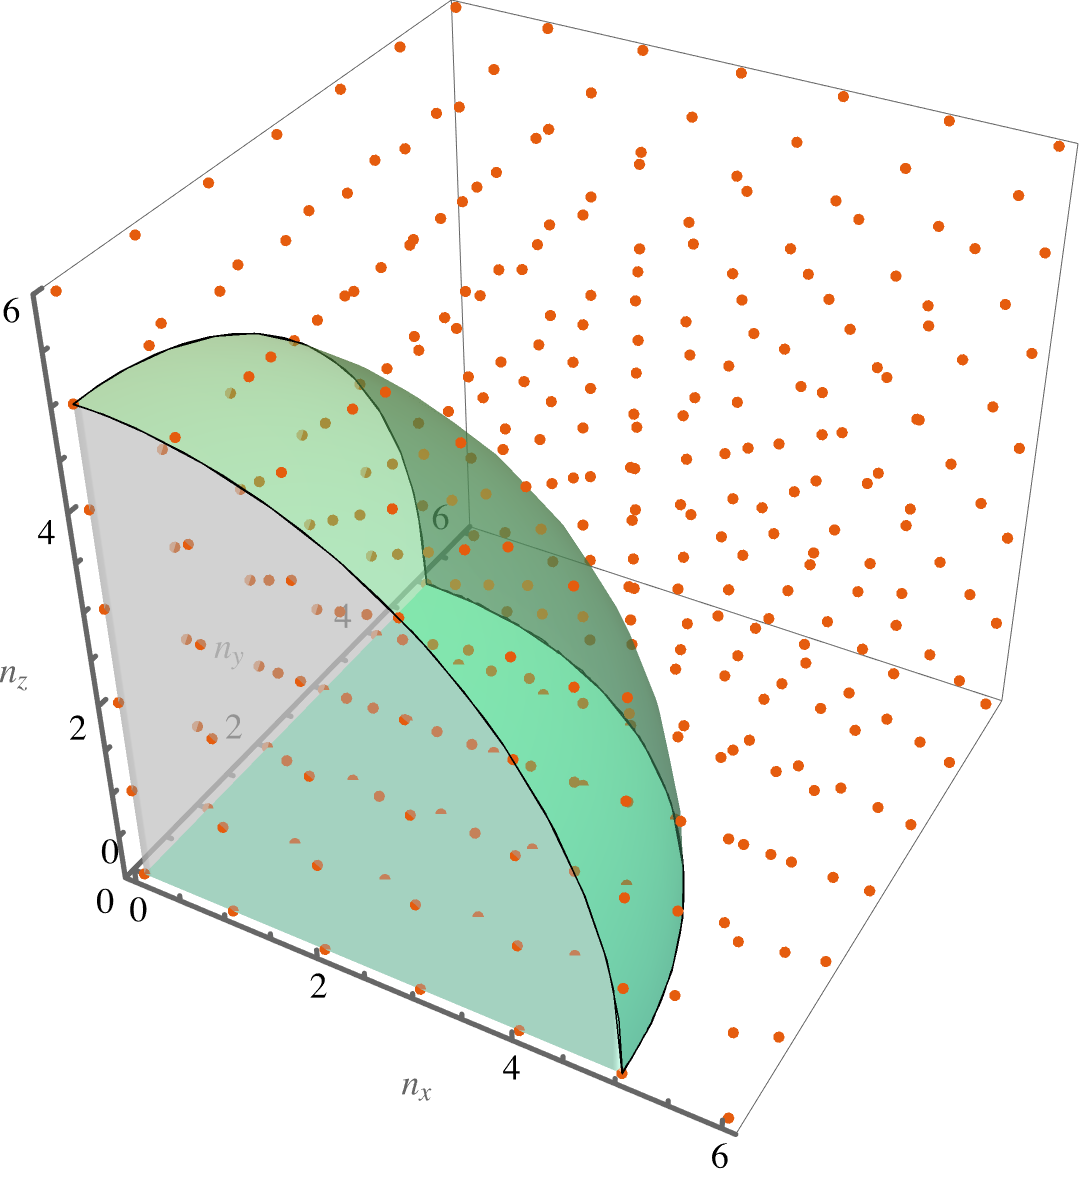
\includegraphics[width=0.6\textwidth]{taimidu.png}
    \caption{系统的状态分布离散而均匀}
    \label{fig:taimidu}
\end{figure}

\begin{justification}{\kaishu 反思与质疑}
    \kaishu \fontsize{11pt}{16pt}
    
    \quad\quad 累计能态密度中需要除以的两个因子 $2^{3N}$ 以及 $N!$ 的原因分别是每个自由度只能取正整数,以及每个粒子不可分辨。并且由于理想气体空间上的稀薄导致的态占据、态分配上的稀薄,相同分子处于同一个态的几率很小,以至于可以忽略不计,所以不需要再添加一个组合因子。

    \quad\quad 那么为什么考虑 $3N$ 个自由度时应当除以 $N!$ 而不是 $(3N)!$ 呢?那是因为是这 $N$ 个粒子不可区分,而不是这 $3N$ 个自由度不可区分,对于每一个粒子来说, $x, y, z$ 都是可以区分的。

    \quad\quad 不过,对于不可分辨粒子设定的合理性,则需要追溯至吉布斯佯谬中来。若认为组成理想气体的各个粒子是可以标号的,首先便会导致推出的熵公式不满足加和性。其次,在考虑同种粒子在同一压强下的混合时,也会推出此时的混合熵正定的矛盾\cite{Pathria}。基于逻辑上的考虑,认为这些粒子具有全同性会使得我们的理论自洽。
\end{justification}

微正则系综以其简单的配容数世界观为基础,帮助我们爬上了统计力学的半山腰。但如果继续向峰巅攀爬将会变得困难,因为微正则系综是一个非常形而上的理论,它对优化参量 $(N,V,E)$ 准确度的要求让我们这些有限的生命望而却步——对于大多数物理系统来说,测量 $(N,V,E)$ 将是一个非常艰巨的任务,更不要说计算出 $\Omega(N,V,E)$ 。

但微正则系综作为我们的理论起点,是值得肯定的,它是我们登山过程中的一条在山脊上延伸的小径。这里先对微正则系综研究方法进行一些总结,然后在下一节中,我们将换个方向——换到沿山谷的石板路上来。

\begin{understanding}{\kaishu 对微正则系综的总结}
\kaishu \fontsize{11pt}{16pt}
\quad\quad 微正则系综以配容数 $\Omega $ 及其对数 $S = k_B \ln \Omega$ 为第一性的量,给了热力学一个完整的逻辑解释。对于经典理想气体,为了计算以 $(N,V,E)$ 为标记的宏观态所能处于的可能的微观态数目,根据粒子能量所可能取值的特点,我们选择将微观态数目与 $3N$ 维状态空间中的球体进行对应。而热力学极限让我们可以合法地使用微分代替寻找方程的整数解,从而得到 $\ln \Omega$ 的渐进表达式。对于量子谐振子系统,则可以使用排列组合直接得到 $\Omega$ 的显式表达式。

\quad\quad 使用微正则系综处理问题可以遵循这样的顺序:
    \begin{enumerate}
        \item 微正则系综的核心量是配容数 $\Omega$
        \item 根据等概率假设,通过对微观态进行简单计数得到 $\Omega(N,V,E)$
        \item $S = k_B \ln \Omega$
        \item 联用热力学公式 $dS = \beta dE + \eta dV + \zeta dN$,偏导数对应相等
    \end{enumerate}

\end{understanding}

\section{正则系综}

前面我们从对热力学的反思中建立了系综理论的基本原理,以 $\Omega$ 为最优化函数, $(N,V,E)$ 为决策变量,通过它们之间的依赖关系我们可以得到系统的所有热力学性质。现在,我们要对微正则系综理论进行反思,并找出一个可以弥补它缺点的解决方案。

使用 $(N,V,E)$ 作为描述系统的最优化过程是一件非常自然的事,因为它们都是广度性质,而使用一些和系统大小成正比的量作为系统的状态参量无疑是非常直观的。然而,这样的直观反而使得我们的理论变得抽象与不切实际:我们很少测量一个物理系统的总能量,并且要想固定它也是很不容易的。

\textcolor{RoyalBlue}{\textbf{\kaishu 问题的根源在于:对微正则系综的三个广度决策变量的测量,不具有实际的可行性。}}  

所以,我们希望找到一个容易测量的,并且和能量具有相同内涵的量来等价地替代 $E$ 作为决策变量的地位——此时我们回想起了理论力学中的勒让德变换。所以我们的目标是:找到一个作用于决策变量 $E$ 的勒让德变换,同时目标函数 $\Omega$ 变为一个新的目标函数 $A$ :
\[
    A = E\frac{\partial \Omega}{\partial E} - \Omega
\]
此时我们再次回想起热力学公式
\[
    dS = \frac{1}{T} dE + \frac{P}{T} dV - \frac{\mu}{T} dN
\]
显然,\textcolor{RoyalBlue}{\textbf{\kaishu 温度 $T$ 就是我们要找的变量}}。随后再对我们想法的一些调整让它能够和热力学建立联系,我们将会看到:变换完全等价地将最优化问题 (\ref*{equ:optimizeI}) 转换成另一个最优化问题:
\begin{equation}\label{equ:optimizeII}
    \begin{split}
        \min A&(N,V,T)\\
        \text{s.t.}\sum n_i = &\mathcal{N},\quad T = T_0
    \end{split}
\end{equation}

其中 $A$ 就是亥姆霍兹自由能,满足 $A = E - TS$ ,以之为核心的即是 \textcolor{RoyalBlue}{\textbf{\kaishu 正则系综}}。

\subsection{正则分布最概然方法}

下面我们来将前面的反思落到实处,此时有必要将系综理论的基本原理再复述一遍:

\textcolor{RoyalBlue}{\textbf{\kaishu 在单一瞬间同时考虑大量系统,他们全部是给定系统的某种“思维复本”——其特性由与原系统一样的宏观态来表征,但极其自然地处在所有各种可能的微观态中}} \cite{Pathria}。

也就是说,我们考虑的不是“这个系统”,而是无数个“这个系统”所组成的更宏大的集合,但集合的元素具有一些关系,并且可能还共同分配了某个想象中的量,并且这个量的分配方式还决定了每个种类的子集所占的比例。

我们考虑的就是这样一件事:把系统看成正则系综的一个成员,然后,由组成系综的 $\mathcal{N}$ 个相同系统去分配该系综总能量 $\mathcal{E}$ ,进而研究这种分配过程的统计学——也就是计算在任意时刻,发现系统处于由能量 $E_r$ 所表征的状态之一的概率 $P_r$ 究竟有多大。

而要固定系统的温度是可以做到的,只需要把系统与一个大热库耦合即可。通过参量$~N~$、$~V~$、$~T~$来描述的系综我们称为正则系综。
当系统$~A~$与一个大热库$~A'~$接触达到平衡时,他们有一个共同的温度$~T~$。它们的能量可以变化,在任意时刻$~t~$,总能量可以处在$~0~$到$~E^{(0)}~$之间的任何值。在某一时刻,系统$~A~$处于由能量$~E_r~$表征的状态下,热库有能量$~E_r'~$,于是有
\[
    E_r + E_r' = E^{(0)} = const
\]
由于热库比系统$~A~$大很多,故$~E_r~$只占$~E^{(0)}~$很少的一部分,即
\[
\frac{E_r}{E^{(0)}} = \left( 1 - \frac{E_r'}{E^{(0)}} \right) \ll 1
\]
用$~\Omega'(E_r')~$记大热库与$~E_r'~$相容的总微观状态数。热库可达到的微观状态数越大,热库具有该能量$~E_r'~$的概率就越大,且由等可能假设,可得相应的概率正比于$~\Omega'(E_r')~$,即
\[
P_r \propto \Omega'(E_r') \equiv \Omega'(E^{(0)} - E_r)
\]
由于$~E_r~$相比$~E^{(0)}~$很小,我们可以对上式在$~E_r' = E^{(0)}~$附近做对数展开,得到

\begin{align*}
\ln \Omega'(E_r') &= \ln \Omega'(E^{(0)}) + \left( \frac{\partial\ln\Omega'}{\partial E'} \right)_{E' = E^{(0)}}(E_r' - E^{(0)}) + \cdots \\
&\simeq const - \beta'E_r
\end{align*}

其中
\[
\left( \frac{\partial\ln\Omega}{\partial E} \right)_{N, V}\equiv\beta
\]
平衡时有$~\beta' = \beta = 1/kT~$. 由展开可求得
\[
P_r \propto \exp(-\beta E_r)
\]
归一得到
\[
P_r = \frac{\exp(-\beta E_r)}{\sum\limits_{r}\exp(-\beta E_r)}
\]
分母的求和遍及了系统$~A~$所有可能达到的状态。

\subsection{}



\begin{justification}{反思与质疑}
\kaishu \fontsize{11pt}{16pt}
    \quad\quad 微正则系综专注于具有同一本征能量的简并微观态,并认为在这些微观态中,没有哪一个是主导,所以引入等概率假设;正则系综则关注具有不同本征能量的各简并集合之间的联系——不同简并集合的大小不同,这些集合之间的比例也有所差异。

    \quad\quad 所以等概率假设与 $e^{\beta E_\nu}$ 并不矛盾,因为一个描述的是简并集合内部的等概率性,一个描述的是这些简并集合之间的比例差异。并且,当我们说出“比例差异”的时候,也就自然地将问题理解为了一个几何概型:具有不同能量的各微观态仍然是等概率的,只是个数不一样。
\end{justification}

\textcolor{RoyalBlue}{\textbf{\kaishu }}











    
    
\section{附录}
\subsection{无穷小正则变换的行列式的绝对值等于 1}
将系统的状态参量 $(q_i,p_i), i = 1,2,\dots n$ 统一表达为 $\xi_\alpha, \alpha = 1,2,\dots 2n$ ,其中前一半是坐标 $q$ ,后一半是动量 $p$ 。引入求和约定,则经典 Poisson 括号可以写为
\[
    [f, g] = \frac{\partial f}{\partial \xi_\alpha}\Omega_{\alpha\beta}\frac{\partial g}{\partial \xi_\beta}
\]
其中
\[
    \Omega = \begin{bmatrix}
        & -I\\
        I&
    \end{bmatrix}_{2n\times 2n}
\]
设正则变换将 $\left \{ \xi \right \}$ 变换为 $\left \{ \xi’ \right \}$ ,雅可比矩阵 $M$ 应为
\[
    M = \begin{bmatrix}
        \frac{\partial \xi_1'}{\partial \xi_1} & \frac{\partial \xi_1'}{\partial \xi_2} & \dots  & \frac{\partial \xi_1'}{\partial \xi_{2n}} \\
        \frac{\partial \xi_2'}{\partial \xi_1} & \frac{\partial \xi_2'}{\partial \xi_2} & \dots  & \frac{\partial \xi_2'}{\partial \xi_{2n}} \\
        \vdots & \vdots &  & \vdots\\
        \frac{\partial \xi_{2n}'}{\partial \xi_1} & \frac{\partial \xi_{2n}'}{\partial \xi_2} & \dots  & \frac{\partial \xi_{2n}'}{\partial \xi_{2n}} \\
    \end{bmatrix}_{2n\times 2n}
\]
由线性代数知识可知,$\text{det}(M\Omega M^T) = \text{det}(M)^2 \text{det}(\Omega) = - \text{det}(M)^2$ ,同时它又可以写为
\begin{align*}
    (M\Omega M^T)_{ij} &= M_{i\alpha}\Omega_{\alpha\beta}M^T_{\beta j}
    = M_{i\alpha}\Omega_{\alpha\beta}M_{j\beta}\\
    &= \frac{\partial \xi'_i}{\partial \xi_\alpha}\Omega_{\alpha\beta}\frac{\partial \xi'_j}{\partial \xi_\beta}\\
    &= [\xi'_i, \xi'_j]_\xi\\
    &= \Omega_{ij}
\end{align*}
最后一个等式用到了正则变换的基本 Poisson 括号不变性。故 $\text{det}(M)^2 = 1$ ,证明完毕。
    
    
\bibliographystyle{plain}
\bibliography{ref}
\end{document}
